\chapter{ Data processing}
\section{kNN}
The dataprocessing will consist of finding the optimal k and smoothing and
DPI which lowers the error rate  This is found by applying knn on different training set,
with different smoothing levels, and DPI. 
For each case will an contour plot be made,
which shows that how each parameter effect each other,
and thereby be useful for deciding which parameter gives the optimal peformance. \\

Different smoothing techniques were applied to the images, such as Gaussian blur and average filters.  
For each were knn applied with different values of, and for each were error rate computed. 
Thereby would it be possible to find the optimal parameter for this sort of problem,
considering the smoothing and value of k. 


\begin{figure}[H]    
	\begin{minipage}[t]{0.30\textwidth}
		\centering
			
\includegraphics[width=0.4\linewidth]{Figure/mikael_8_2_dpi100_k1.png}
			\caption{DPI = 100 , kernel size = 1}
			\label{fig:dpi_100_1}
	\end{minipage}
	\hspace{\fill}	
	\begin{minipage}[t]{0.30\textwidth}
		\centering
			
\includegraphics[width=0.4\linewidth]{Figure/mikael_8_2_dpi100_k3.png}
			\caption{DPI = 100 , kernel size = 3}
			\label{fig:dpi_100_3}
	\end{minipage}
	\hspace{\fill}
	\begin{minipage}[t]{0.30\textwidth}
		\centering
			
\includegraphics[width=0.4\linewidth]{Figure/mikael_8_2_dpi100_k5.png}
			\caption{DPI = 100 , kernel size =5}
			\label{fig:dpi_100_5}
	\end{minipage}
\vspace*{0.5cm} % (or whatever vertical separation you prefer)	
	\begin{minipage}[t]{0.30\textwidth}
		\centering
			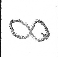
\includegraphics[width=0.4\linewidth]{Figure/mikael_8_2_dpi300_k1.png}
			\caption{DPI = 300 , kernel size = 1}
			\label{fig:dpi_300_5}
	\end{minipage}
\hspace{\fill}	
	\begin{minipage}[t]{0.30\textwidth}
		\centering
			
\includegraphics[width=0.4\linewidth]{Figure/mikael_8_2_dpi300_k5.png}
			\caption{DPI = 300 , kernel size = 5}
			\label{fig:dpi_300_9}
	\end{minipage}	
\hspace{\fill}	
	\begin{minipage}[t]{0.30\textwidth}
		\centering
			
\includegraphics[width=0.4\linewidth]{Figure/mikael_8_2_dpi300_k9.png}
			\caption{DPI = 300 , kernel size = 9}
			\label{fig:dpi_300_9}
	\end{minipage}	
\caption{Effect of smoothing using average filter with different kernel sizes}
\label{fig:average_filter}
\end{figure}

It can be seen based on figure \ref{fig:average_filter} that the
 filter does have an impact on how clear the digit can be visually
 recognized, and that the higher the dpi values is,
  the better visual information do one get. 
Using this form of smoothing were different valued kNN applied,
at for which each were compared to an testset to see how accurately it could classify the digits. 

\begin{figure}[H]
	\centering
		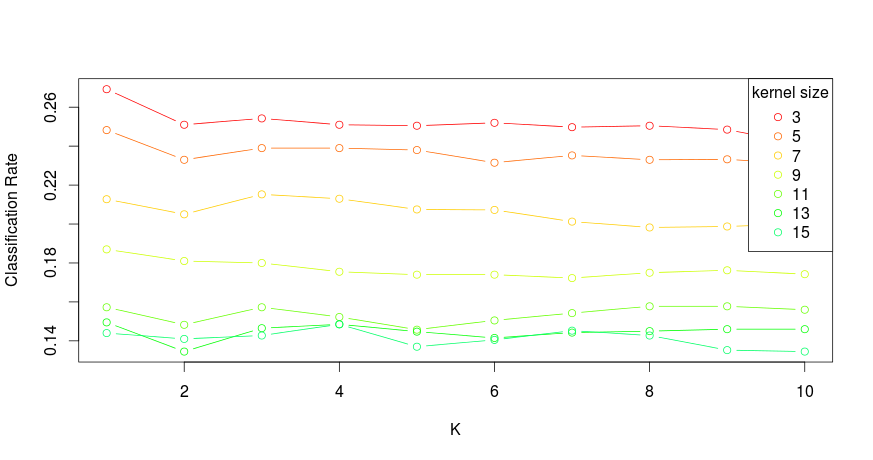
\includegraphics[width = \textwidth]{Figure/data_100_15_10.png}
		\caption{Tested on images with 100 dpi}
		\label{fig:data_100}
\end{figure}

\begin{figure}[H]
	\centering	
		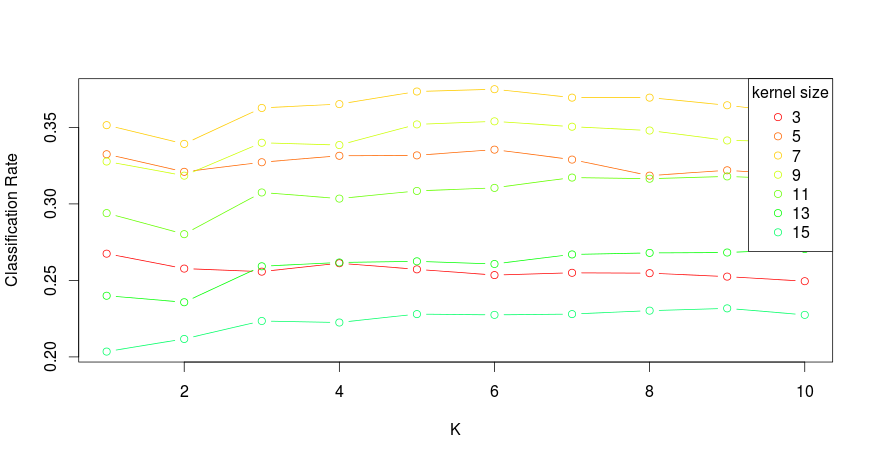
\includegraphics[width = \textwidth]{Figure/data_200_15_10.png}
		\caption{Tested on images with 200 dpi}
		\label{fig:data_200}
\end{figure}

\begin{figure}[H]
	\centering
		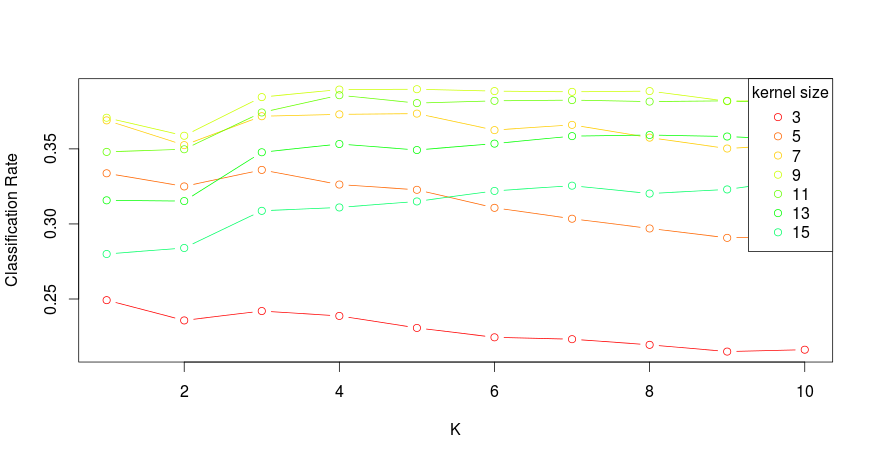
\includegraphics[width = \textwidth]{Figure/data_300_15_10.png}
		\caption{Tested on images with 300 dpi}
		\label{fig:data_300}
\end{figure}

The graphs in figure \ref{fig:data_100} , \ref{fig:data_200}  and \ref{fig:data_300} 
 shows that the images scanned with 300 DPI gives the highest classification rate,
which as previously stated was seen as the once who gave clearer images as smoothing were applied.
 The graphs shows that classification peaks for 200 DPI when applying a kernel at size 3,
 for 200 dpi peaks it at kernel size 7, and for 300 dpi peaks it at kernel size 9,
 So in general increases the classification rate, as the dpi increases with the kernel size.
 The best perfomance can by found from the images scanned with 300 dpi,
 but one could question whether the peformance of it is satisfiable. 

\begin{figure}[H]    
	\begin{minipage}[t]{0.30\textwidth}
			\centering
			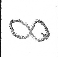
\includegraphics[width=0.4\linewidth]{Figure/mikael_8_2_dpi300_k15_sig_01.png}
			\caption{kernelsize = 15 $\sigma$ = 0.1}
			\label{fig:dpi_300_k_9_s_0.1}
	\end{minipage}
	\hspace{\fill}	
	\begin{minipage}[t]{0.30\textwidth}
		\centering
			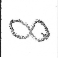
\includegraphics[width=0.4\linewidth]{Figure/mikael_8_2_dpi300_k15_sig_04.png}
			\caption{kernelsize = 15 $\sigma$ = 0.4}
			\label{fig:dpi_300_k_9_s_0.4}
	\end{minipage}
	\hspace{\fill}
	\begin{minipage}[t]{0.30\textwidth}
		\centering
			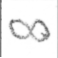
\includegraphics[width=0.4\linewidth]{Figure/mikael_8_2_dpi300_k15_sig_07.png}
			\caption{kernelsize = 15 $\sigma$ = 0.7}
			\label{fig:fig:dpi_300_k_9_s_0.7}
	\end{minipage}
\caption{Effect of smoothing using gaussian filter with different sigma values}
\label{fig:gaussian_filter}
\end{figure}

As an alternative to the average filter could an gaussian filter be used as shown
 in figure \ref{fig:gaussian_filter}. 
 The perfomance of the filter shows, seem to visually remove more noise than the previous,
 and would potentially also have provided at better classification rate than the other one. 



